%%%%%%%%%%%%%%%%%%%%%%%%%%%%%%%%%%%%%%
%%  
%% Chapter 1: Introduction to heterogeneous computing
%%
%%%%%%%%%%%%%%%%%%%%%%%%%%%%%%%%%%%%%%

\def\ArtDir{01.HeteroComp/figures}%

\chapter{Heterogeneity and the future of computing}
\label{chapter:heterogeneity}

\section{What is Heterogeneous computing and why everyone will be doing it}

\section{The basic building blocks of modern computing}

\begin{itemize}
\item Introduce a set of standard processors.
\item  the CPU: the multiprocessor and cache coherent memory
\item  the SIMD or Vector Unit: lock-step execution across vector lanes
\item  the GPU:  Index space, kernels, work-items and work-groups
\end{itemize}

\subsection{Introduce Cache coherent shared memory machine. SMP model.}
Introduce what a standard CPU looks like. This is the host processor.

\subsection{Introduce GPU model}
When discussing parallel programming models in general, is it sometimes important to distinguish between concurrent concepts in the programming model and parts of the hardware.
On CPUs for instance, parallel items called perhaps ``threads'' are assigned to run on physical parts of the CPU called perhaps ``cores''.
This correspondence is not necessarily unique, and parallelism expressed in the programming model may be assigned physical components of the processor in a number of ways.

OpenMP does not give sufficient terminology to name the underlying hardware of a given abstract device, and so to help throughout this book, we define an underlying target device using terminology borrowed from another open-standard programming model called OpenCL (from Khronos).
This is no criticism of OpenMP for it is typically an implementation detail on how the parallel concepts in OpenMP might correspond to physical, real-life hardware.
However in our situation, it is helpful to speak in terms regarding expressing parallelism in OpenMP differently to how that might correspond at run-time to the physical hardware.

A target device is constructed with a hierarchical structure of hardware.
The target device is built from a number of Compute Units (CUs)\index{Compute Unit}.
Each Compute Unit is formed from a number of Processing Elements (PEs)\index{Processing Element}.
The Processing Elements themselves are the hardware that can execute the program instructions, and are organised into Compute Units.
Processing Elements can operate independently but there is normally close ties with the other Processing Elements within the Compute Unit.
There is normally no (or little) interaction between Processing Elements in different Compute Units.
In particular, Processing Elements are not allowed to communicate with each other unless they reside in the same Compute Unit.

Each Processing Element may be able to execute vector (SIMD) instructions\index{SIMD}, and so might contain the requisite hardware for this.
The number of data elements the SIMD instructions process is called the width.
We call the location of each data item within the instruction a SIMD lane\index{SIMD lane}.

This three level hierarchy is shown in Figure \ref{figure:target_device_hierarchy}.
The parallel concepts in the OpenMP programming model will be assigned to Compute Units, Processing Elements, and SIMD lanes.

\begin{figure}[t]
\centerline{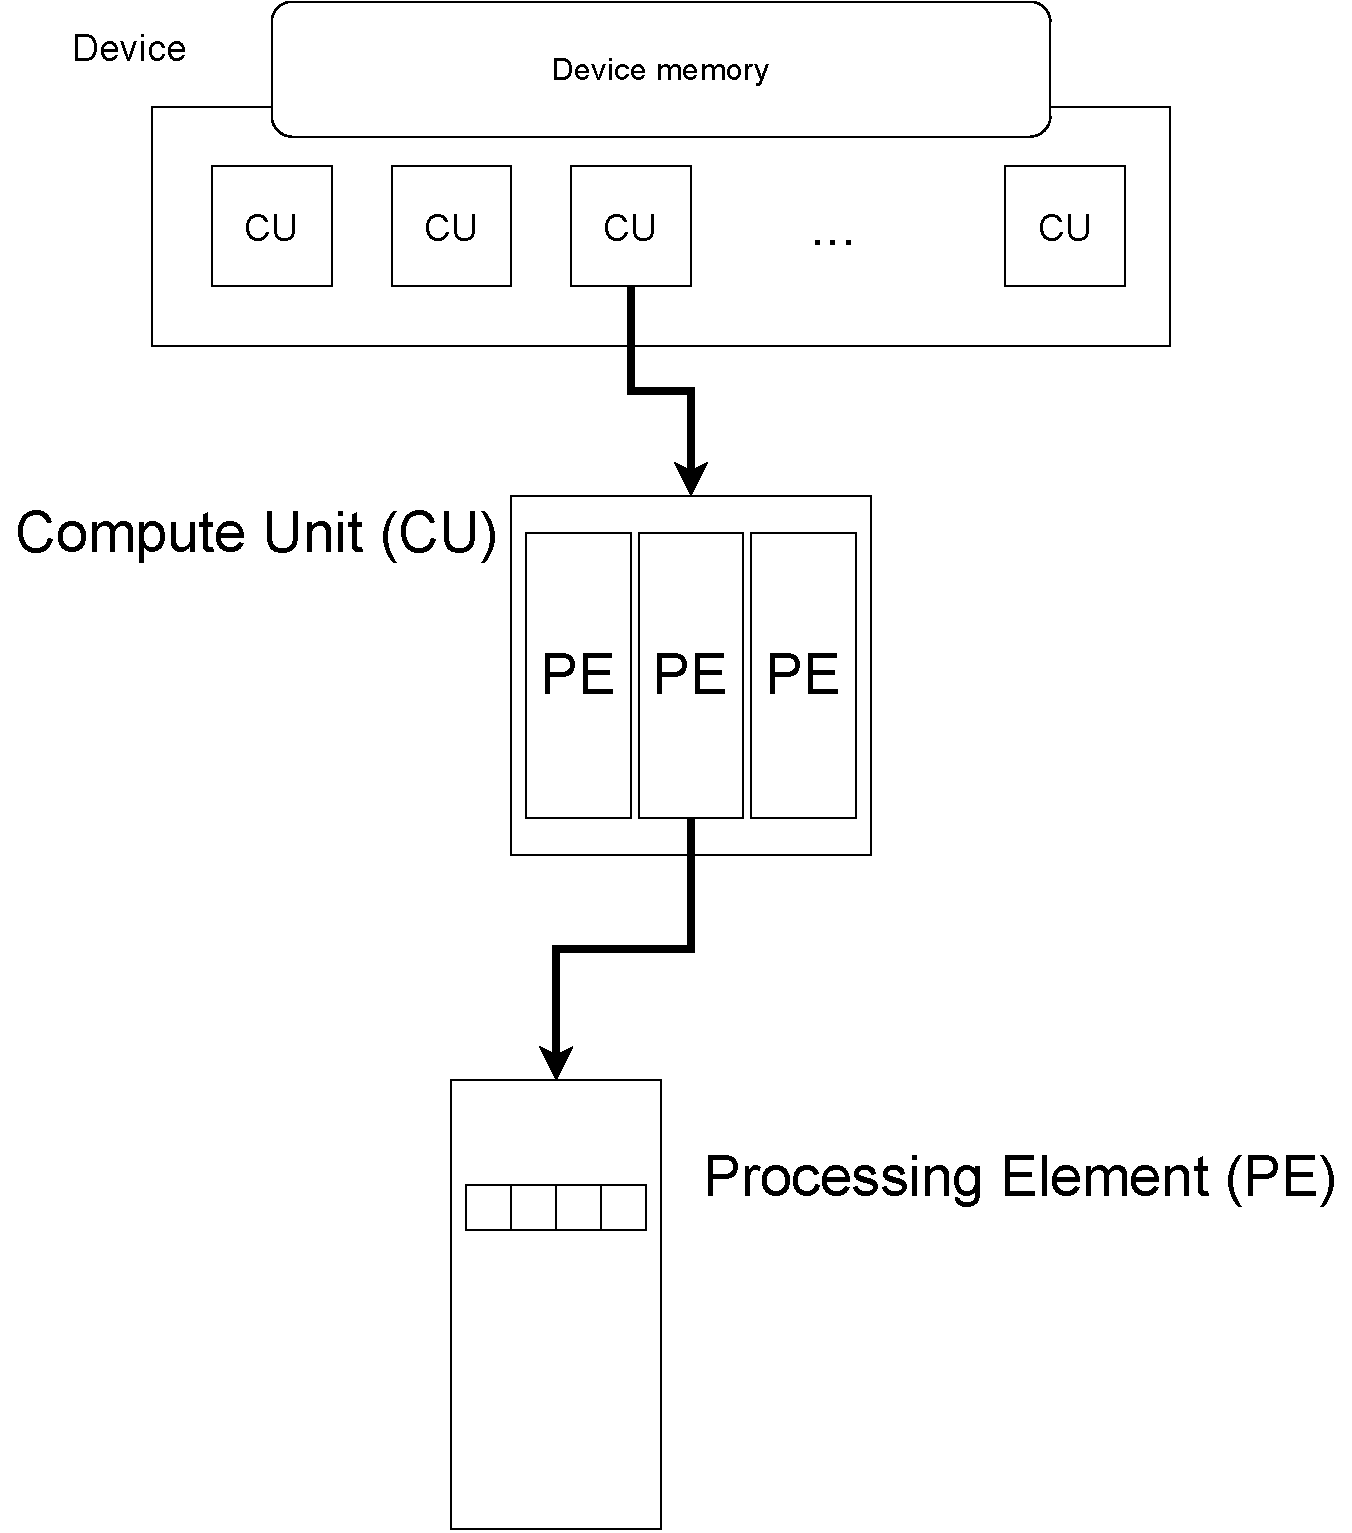
\includegraphics[width=200pt]{\ArtDir/target_device.pdf}}
\caption{A target device is formed of a number of Compute Units (CU). Each of these Compute Units is formed of a number of Processing Elements (PE), which may be able to execute vector (SIMD) instructions.}
\label{figure:target_device_hierarchy}
\end{figure}

The device memory is shared and available to all of the hierarchy of hardware.
Each Compute Unit might in addition provide a layer of memory available only to those Processing Elements contained within it.
This we will call (as in OpenCL) the local memory\index{local memory}.
The Processing Elements in each Compute Unit can access this memory, however it is not accessible by Processing Elements outside the Compute Unit.
We will address using this local memory in OpenMP in Section~\ref{sec:team_only_memory}.

This book will show how to program a device like this, such as GPU, using OpenMP.
In later chapters, we include case studies to show the abstract device model and the concepts in OpenMP come together and are applied to real hardware.


\section{Why you need OpenMP: a single code-base for heterogeneous hardware}

\section{Templates for use in formatting the rest of the book.}

Here is how we handle a code fragment embedded in text.
Consider a simple program that adds two vectors, \code{a} and \code{b}.
\begin{verbatim}
      for (i = 0; i < N; i++) { 
         a[i] = a[i] + b[i];
      }
\end{verbatim}  

For longer code fragments, we put the code in a proper figure.  For example, consider figure~\ref{code:vaddSPMD}

\begin{CodeExample}%
{\textbf{SPMD parallel vector add program} -- \small
Create a team of threads and assign one chunk of loop iterations
to each thread.
}%
{code:vaddSPMD}
\begin{lstlisting}
// OpenMP parallel region and SPMD pattern
#pragma omp parallel
{
   int id, i, Nthrds, istart, iend;
   id = omp_get_thread_num();
   Nthrds = omp_get_num_threads(); 
   istart = id * N / Nthrds;
   iend = (id + 1) * N / Nthrds;
   if (id == Nthrds - 1) iend = N; 
   for (i = istart; i < iend; i++) {
      a[i] = a[i] + b[i];
   }
}
\end{lstlisting}
\end{CodeExample} 



When we have specific constructs to introduce, we use a table with marcros for the constructs themselves.  This way we can make 
sure that we use consistent fonts and styles across the entire book.  Take a look at table~\ref{tab:omp_for} for a good example.

\begin{table}[!htbp]
\centering
\caption{\textbf{A basic worksharing-loop construct in C/C++ and Fortran} 
-- \small
The worksharing-loop construct shares the iterations of a loop among
a team of threads.  The loop is called \texttt{for} in C and \texttt{DO} in Fortran.
Fortran is not block structured, so we need an \texttt{END DO} directive.
Optional clauses give the programmer more control
over the loop construct and include \texttt{schedule}, \texttt{reduction}, and 
\texttt{nowait}. We will discuss these clauses later in this chapter.  Additional clauses define storage attributes 
of the variables used in the worksharing-loop.  We will cover those in 
Chapter~\ref{ch:dataEnv}.  
}
\label{tab:omp_for}
\begin{tabular}{|l|} \hline
\ompbcfor \ompclauses \\ 
%\hspace{5mm} \{   \\
\hspace{5mm} for-loop \\      
%\hspace{5mm} \}    \\           
\hline
\ompbfdo \ompclauses  \\ 
%\hspace{5mm} \{   \\
\hspace{5mm} do-loop   \\
%\hspace{5mm} \}   \\ 
\ompbfdoend \textit{ [nowait] } \\   
                  
\hline

\end{tabular}
\end{table}

Here is an index entry:  Moore's law\index{Moore's law} and a citation Dennard scaling\index{Dennard scaling}~\cite{Dennard}, 


There are some open questions concerning what we need to cover.
\begin{itemize}
\item Do we need to include \code{declare simd}?  Is that enabled for a GPU?  
\item Do we need to discuss the variant directives?  If they are 
important for GPU programmers, then we probably need to. Likewise for assumes and assume.  
\item Does the scan directive apply to GPUs?  
\item Does tile and unroll apply to GPUs?  
\item Do memory spaces apply to GPUs?
\end{itemize}

We will also need to cover a set of internal control variables and where appropriate a set of environment variables.

\begin{table}[h!]
\centering
\caption{All the pragmas we will cover in the book and the chapters where we will cover them}
\label{YourLabel}
%%%%%%%%%%%%%%%%%%%%%%%%%%%%%%%%%%%%%%
%%  
%% The table contains OpenMP pragmas we'll cover in the book
%%
%% To use this in one of our chapters, use the latex command
%%         \begin{table}[h!]
%%          \centering
%%          \caption{Your caption}
%%           \label{YourLabel}
%%           \input{\SubDir/CommonCoreTab.tex}
%%           \end{table}
%%
%%  where the macro \SubDir is defined at the top of each chapter and 
%%  specifies where the source for the book resides.   
%%
%%%%%%%%%%%%%%%%%%%%%%%%%%%%%%%%%%%%%%

\begin{tabular}{|l|l|l|l|}
\hline
\textbf{OpenMP pragma}  & \textbf{Concepts} & \textbf{Chapter} & \textbf{Structure} \\
\hline
%============================================================
\Code{#pragma omp target}                & offload onto a device  & \S\ref{chapter:target} & Core \\ 
\hline 
\Code{#pragma omp teams}                & Create a league of teams & \S\ref{sec:teams} & Core \\
\hline
\Code{#pragma omp distribute}            & Map loops onto a league & \S\ref{ssec:teams_distribute} & Advanced (on its own, favor combined) \\
\hline
\Code{#pragma omp target data}            & Create a device data region & \S\ref{ssec:target_data} & Core \\
\hline
\Code{#pragma omp target enter data}  & Enter a device data region & \S\ref{ssec:target_enter_exit_data} & Core \\
\hline
\Code{#pragma omp target exit data}  & Exit a device data region & \S\ref{ssec:target_enter_exit_data} & Core \\
\hline
\Code{#pragma omp target update}  & Update data between host/device & \S\ref{ssec:target_update} & Core \\
\hline
\Code{#pragma omp loop}  & Concurrent loop iterations & \S\ref{sec:loop} & Core \\
\hline
\Code{#pragma omp requires} & OMP features required & \S\ref{sec:usm} & Core/Advanced \\
\hline
\Code{#pragma omp declare target} & declares items are mapped to a device & \S\ref{ssec:declare_target} & Advanced \\
\hline
\Code{#pragma declare mapper} & user defined mapers & \S\ref{sec:mapper} & Advanced \\
\hline
\Code{#pragma omp interop} & Interoperability with foreign contexts & \S\ref{sec:interop} & Advanced \\
\hline
\Code{teams loop}    & combined construct & \S\ref{sec:loop} & Core \\
\hline
\Code{teams distribute}  & combined  construct & \S\ref{ssec:teams_distribute} & Core \\
\hline
\Code{teams distribute simd}  & combined  construct & XX & Advanced (not useful?) \\
\hline
\Code{teams distribute parallel for} & combined  construct & XX & Advanced \\
\hline
\Code{teams distribute parallel for simd} & combined  construct & \S\ref{sec:bud} & Core \\
\hline
\Code{target parallel}    & combined construct & XX & Advanced \\
\hline
\Code{target simd}    & combined construct & XX & Advanced \\
\hline
\Code{target parallel for}    & combined construct & XX & Advanced \\
\hline
\Code{target parallel for simd}    & combined construct & XX & Advanced \\
\hline
\Code{target parallel loop}    & combined construct & XX & Advanced (N/A?) \\
\hline
\Code{target teams }    & combined construct & XX & Advanced \\
\hline
\Code{target teams loop}    & combined  construct & \S\ref{sec:loop} & Core \\
\hline
\Code{target teams distribute}  & combined  construct & XX & Advanced \\
\hline
\Code{target teams distribute simd}  & combined  construct & XX & Advanced (N/A?) \\
\hline
\Code{target teams distribute parallel for} & combined  construct & XX & Advanced \\
\hline
\Code{target teams distribute parallel for simd} & combined  construct & \S\ref{sec:bud} & Core \\
\hline
\end{tabular}

Comment: best practice often favors the combined constructs (distribute must be strictly nested).

Comment: often the combined construct falls out naturally from explaining what the bits mean.



 \end{table}

\begin{table}[h!]
\centering
\caption{All the clauses we will cover in the book and the chapters where we will cover them}
\label{YourLabel}
%%%%%%%%%%%%%%%%%%%%%%%%%%%%%%%%%%%%%%
%%  
%% The table contains every single clause we will cover from specification
%%
%% To use this in one of our chapters, use the latex command
%%         \begin{table}[h!]
%%          \centering
%%          \caption{Your caption}
%%           \label{YourLabel}
%%           \input{\SubDir/CommonCoreTab.tex}
%%           \end{table}
%%
%%  where the macro \SubDir is defined at the top of each chapter and 
%%  specifies where the source for the book resides.   
%%
%%%%%%%%%%%%%%%%%%%%%%%%%%%%%%%%%%%%%%

\begin{tabular}{|l|l|l|l|}
\hline
\textbf{OpenMP clauses}  & \textbf{Constructs} & \textbf{Chapter} & \textbf{Structure} \\
\hline
%============================================================
\Code{private}                   & teams, distribute, simd, loop, target & \S\ref{sssec:data_sharing} & Core \\
\hline
\Code{firstprivate}              & teams & \S\ref{sssec:data_sharing} & Core \\
\hline
\Code{lastprivate}              & distribute, simd, loop   & \S\ref{sssec:data_sharing} & Advanced \\
\hline
\Code{shared}           & teams & \S\ref{sssec:data_sharing} & Core (concept) / Advanced (clause itself)\\
\hline
\Code{reduction}           & teams, parallel & \S\ref{sec:reduction} and \S\ref{sec:target_reductions} & Core \\
\hline
\Code{allocate}           & (allocator for private variables) target, teams, distribute & XX & Advanced (N/A?) \\
\hline
\Code{default}           & teams & XX & Advanced \\
\hline
\Code{num_teams}           & teams & \S\ref{ssec:gpu_specific_mapping} & Advanced \\
\hline
\Code{thread_limit}           & target, teams & XX & Advanced (N/A?) \\
\hline
\Code{reduction}    & simd, loop & see above & Core \\
\hline
\Code{in\_reduction}    & target & \S\ref{sec:in_reduction} & Advanced \\
\hline
\Code{collapse}      & simd, loop & \S\ref{ssec:fork_join} & Core \\
\hline
\Code{dist\_schedule}    & distribute & \S\ref{ssec:teams_distribute} & Core (but not recommended) \\
\hline
\Code{order}                   & distribute, loop & XX & Advanced \\
\hline
\Code{bind}              & loop & XX & Advanced (esoteric) \\
\hline
\Code{if}            & simd, target, target data, target enter data, target exit data & \S\ref{sec:if_clause} & Advanced (might be Core?)\\
\hline
\Code{safelen}   & simd & XX & N/A \\
\hline
\Code{simdlen}   & simd & XX & Advanced? (N/A) \\
\hline
\Code{aligned}   & simd & XX & N/A \\
\hline
\Code{linear}      & simd & XX & N/A \\
\hline
\Code{nontemporal}   & simd & XX & N/A \\
\hline
\Code{map}      & target, target data, target enter data, target exit data, declare mapper & \S\ref{ssec:map_clause} & Core \\
\hline
\Code{use\_device\_ptr}    & target data (interop) & XX & Advanced \\
\hline
\Code{is\_device\_ptr}    & target (interop, alloc APIs) & \S\ref{sec:alloc_apis} & Advanced \\
\hline
\Code{use\_device\_addr}     & target data (interop) & XX & Advanced \\
\hline
\Code{has\_device\_addr}     & target (interop, alloc APIs) & \S\ref{sec:alloc_apis} & Advanced \\
\hline
\Code{uses\_allocaters}    & target data & XX & Advanced (esoteric) \\
\hline
\Code{device}           & target,target data, target enter data, target exit data, interop & \S\ref{sec:host_device_model} and multi-gpu section & Core \\
\hline
\Code{depend}      & target,target enter data, target exit data, interop & \S\ref{chapter:async} & Core \\
\hline
\Code{nowait}     & target,target enter data, target exit data, interop & \S\ref{chapter:async} & Core \\
\hline
\Code{to/from}    & update & \S\ref{ssec:target_update} & Core \\
\hline
\Code{to}    & declare\_target & \S\ref{ssec:declare_target} & Advanced \\
\hline
\Code{link}    & declare\_target & \S\ref{ssec:declare_target} & Advanced \\
\hline
\Code{device\_type}   & declare\_target & \S\ref{ssec:declare_target} & Advanced \\
\hline
\Code{indirect}     & declare\_target & \S\ref{ssec:declare_target} & Advanced \\
\hline
\Code{init}      & interop & XX & Advanced \\
\hline
\Code{destroy}   & interop & XX & Advanced \\
\hline
\Code{use}       & interop & XX & Advanced \\
\hline
\end{tabular}

Comment: simd clauses same as from Next Steps book.






 \end{table}
 
\begin{table}[h!]
\centering
\caption{All the runtime functions we will cover in the book and the chapters where we will cover them}
\label{YourLabel}
%%%%%%%%%%%%%%%%%%%%%%%%%%%%%%%%%%%%%%
%%  
%% The table contains every single runtime function we will cover from specification
%%
%% To use this in one of our chapters, use the latex command
%%         \begin{table}[h!]
%%          \centering
%%          \caption{Your caption}
%%           \label{YourLabel}
%%           \input{\SubDir/CommonCoreTab.tex}
%%           \end{table}
%%
%%  where the macro \SubDir is defined at the top of each chapter and 
%%  specifies where the source for the book resides.   
%%
%%%%%%%%%%%%%%%%%%%%%%%%%%%%%%%%%%%%%%

\begin{tabular}{|l|l|}
\hline
\textbf{OpenMP functions,}  & Chapter \\
\hline
%============================================================
\Code{int omp\_get\_team\_size()}      & XX \\
\hline
\Code{int omp\_get\_num\_teams()}       & XX   \\
\hline
\Code{int omp\_get\_team\_num()}       & XX   \\
\hline
\Code{void omp\_set\_num\_teams()}       & XX    \\
\hline
\Code{int omp\_get\_max\_teams()}      & XX    \\
\hline
\Code{void omp\_set\_teams\_thread\_limit()}     & XX    \\
\hline
\Code{int omp\_get\_teams\_thread\_limit()}      & XX    \\
\hline
\Code{int omp\_get\_teams\_thread\_limit()}      & XX    \\
\hline
\Code{int omp\_pause\_resource()}      & XX    \\
\hline
\Code{int omp\_pause\_resource\_all()}    & XX    \\
\hline
\Code{int omp\_get\_num\_procs()}     & XX    \\
\hline
\Code{void omp\_set\_default\_device()}    & XX    \\
\hline
\Code{int omp\_get\_default\_device()}          & XX    \\
\hline
\Code{int omp\_get\_num\_devices()}         & XX    \\
\hline
\Code{int omp\_get\_device\_num()}       & XX    \\
\hline
\Code{int omp\_is\_initial\_device()}         & XX    \\
\hline
\Code{int omp\_get\_initial\_device()}          & XX    \\
\hline
\Code{void* omp\_target\_alloc()}        & XX    \\
\hline
\Code{void omp\_target\_free()}        & XX    \\
\hline
\Code{int omp\_target\_is\_present()}           & XX    \\
\hline
\Code{int omp\_target\_is\_axxessible()}          & XX    \\
\hline
\Code{int omp\_target\_memcpy()}          & XX    \\
\hline
\Code{int omp\_target\_memcpy_rect()}          & XX    \\
\hline
\Code{int omp_target_memcpy_async()}          & XX    \\
\hline
\Code{int omp_target_memcpy_rect_async()}          & XX    \\
\hline
\Code{int omp_target_associate_ptr()}          & XX    \\
\hline
\Code{omp_target_disassociate_ptr()}          & XX    \\
\hline
\Code{void *omp_get_mapped_ptr()}          & XX    \\
\hline
\Code{int omp_get_num_interop_properties()}          & XX    \\
\hline
\Code{int omp_get_num_interop_properties()}          & XX    \\
\hline
\Code{void *omp_get_interop_ptr()}          & XX    \\
\hline
\Code{void *omp_get_interop_ptr()}          & XX    \\
\hline
\Code{const char* omp_get_interop_name()}          & XX    \\
\hline
\Code{const char* omp_get_interop_type_desc()}          & XX    \\
\hline
\Code{const char* omp_get_interop_rc_desc ()}          & XX    \\
\hline
\end{tabular}




 \end{table}
 
\begin{table}[h!]
\centering
\caption{All the internal control variables and associated environment variables we will 
cover in the book and the chapters where we will cover them}
\label{YourLabel}
%%%%%%%%%%%%%%%%%%%%%%%%%%%%%%%%%%%%%%
%%  
%% The table contains OpenMP ICVs and Env Vars we'll cover in the book
%%
%% To use this in one of our chapters, use the latex command
%%         \begin{table}[h!]
%%          \centering
%%          \caption{Your caption}
%%           \label{YourLabel}
%%           \input{\SubDir/CommonCoreTab.tex}
%%           \end{table}
%%
%%  where the macro \SubDir is defined at the top of each chapter and 
%%  specifies where the source for the book resides.   
%%
%%%%%%%%%%%%%%%%%%%%%%%%%%%%%%%%%%%%%%

\begin{tabular}{|l|l|l|}
\hline
\textbf{ICV}  & Env var & Chapter \\
\hline
%============================================================
\Code{thread-limit-var}                & \Code{OMP\_THREAD\_LIMIT} & XX \\ 
\hline 
\Code{default-device-var}                & \Code{OMP\_DEFAULT\_DEVICE} & XX \\
\hline
\Code{target-offload-var}            & \Code{OMP\_TARGET\_OFFLOAD} & XX \\
\hline
\Code{nteams-var}            & \Code{OMP\_NUM\_TEAMS} & XX \\
\hline
\Code{teams-thread-limit-var}  & \Code{OMP\_TEAMS\_THREAD\_LIMIT} & XX \\
\hline
\end{tabular}



 \end{table}


%-----------------------------------------------------------------------
%------------------------- From Next Step ------------------------------
%-----------------------------------------------------------------------
\section{From The Next Step Chapter 5}

Specialized accelerator processors, which dramatically improve the performance
of some computations, are proliferating, and general-purpose processors are
now very often connected to some type of accelerator.  
The popularity of these heterogeneous architectures across all types of
computing has had a noticeable impact on the development of software.  

To exploit these systems, developers must write software that executes various
regions of code on different types of devices.  There are many reasons for
wanting to do this but very often the motivation is to accelerate
computationally intensive loop nests.  

However, the programming models for these systems are difficult to use.
Often code modules are written twice, once for the general-purpose
processor and then again for the accelerator.  The accelerator version is often
written in a lower-level, accelerator-specific language.  The result is the
undesirable software maintenance problem of keeping two versions of code, which
implement the same algorithm, synchronized.

The \OMP\ Language Committee recognized the need to make it easier to program
heterogeneous architectures and set about to extend \OMP\ to support these types
of systems \cite{Beyer2011}.  The results of this work were initially released
in \OMPfourzero\ and updated in \OMPfourfive.

Software developers can use \OMP\ to program accelerators in a higher-level
language and maintain one version of their code, which can run on either an
accelerator or a general-purpose processor.  In this chapter, we present the
syntax for and describe how to use the \OMP\ \emph{device constructs} and
related runtime functions that were added to support heterogeneous
architectures. 

%What was needed is a programming model that could...
%Given the popularity of heterogeneous systems across all types of computing,

%There is a place here for \OMP\ to make these software packages more
%maintainable and portable.  We hope that in the future, as the latest versions
%of \OMP\ are implemented in more compilers, software developers will leverage
%the \OMP\ device constructs and develop one version of their code that can run
%anywhere, including on accelerators.

%There is a place here for \OMP\ to make these software packages more
%maintainable and portable.  We hope that in the future, as the latest versions
%of \OMP\ are implemented in more compilers, 
